\section{Check Your Units!}

\begin{comment}
This lab is more of a worksheet than it is a lab.  But I've used versions of if in my 131 classes for a while, so I thought it was time to include it here in the lab manual for others as well.  I usually do this right after forces, so they have some idea of units of force, mass, and coefficients of friction.  Come to think of it, this might even be useful just as a homework assignment; students can probably do it on their own.  --Matt Trawick, 7/2015

\end{comment}

\makelabheader %(Space for student name, etc., defined in master.tex or labmanual_formatting_commands.tex)

%\rule{1.0in}{0.1pt}

\vspace{0.1in}
\textbf{Objective:} to learn how examining units can help you check your answers and locate algebra mistakes. 
\bigskip

1. What is 2 cm plus 3 cm?
\vspace{0.2in}

2. What is 1 foot plus 3 inches?
\vspace{0.2in}

3. What is 1 foot plus 3 pounds?
\vspace{0.2in}

4. What is 1 foot plus $\sin 30 ^\circ $?
\vspace{0.2in}

\textit{For two of the questions above, the correct answer is actually "complete nonsense," because you can't add two quantities that have fundamentally different units, like length and velocity.  The next part of this lab shows how you can use this principle to check your work when you solve problems.}

5. Anna has solved a problem where she found the tension in a string to be 
$$T = m_1g - \frac{\mu_k m_1}{m_2} F_A (1 - \sin\theta).$$ 
She checks her answer with Bob, who found 
$$T = m_1g - \frac{\mu_k m_1}{m_2} F_A (m_1 - \sin\theta).$$ 
Since they disagree, at least one of them has to be wrong.  Who is definitely wrong, and why?
\vspace{0.7in}

6. On the next page, a student has solved a fairly complicated problem involving rotational motion, finding the acceleration $a_1$ of a falling mass. (Don't worry about understanding the problem or the physics for now.)  Look at the final answer on line 15, and use what you know about units to decide whether the final answer could be correct.  How do you know?
\vspace{0.7in}

7. It turns out that there must be an algebra boo-boo somewhere on the page that we will have to find.  But instead of re-deriving every line, we'll pick just one line in the middle (we'll try line 11) to see whether the units there are okay.  Are they?
\vspace{0.4in}

8. Now that you know the mistake has to be someplace between line 11 and line 15, is line 13 okay or not okay?
\vspace{0.2in}

9. Find the algebra mistake and write the correct answer for $a_1$ below.
\vspace{0.5in}

\newpage

\begin{center}
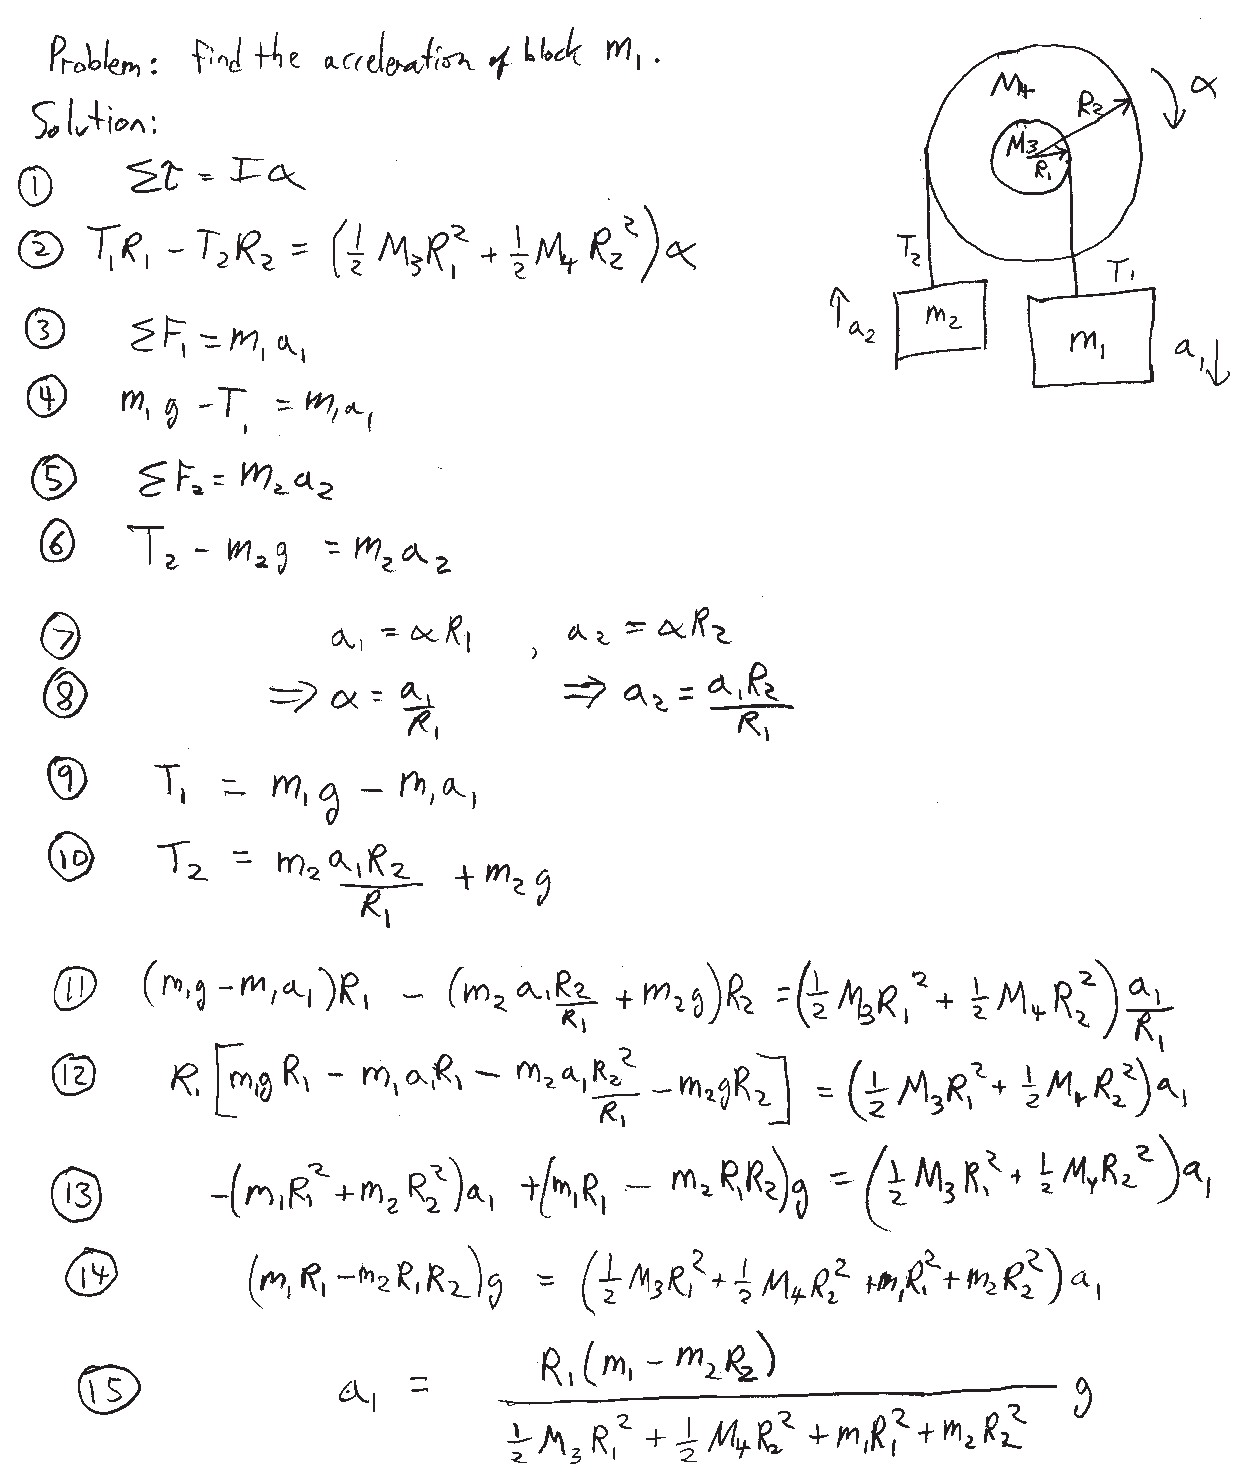
\includegraphics[width=0.99\textwidth]{check_your_units/find_the_error_using_units2.eps}
\end{center}

\textit{You can use what you know about units to quickly locate algebra mistakes in complicated problems like the one above.}



